\section{Experiments}
\label{sec:exp}

\paragraph{Protocol.}
The main split trains on campaigns A, B and C (June and July, \EpTrainABC\ episodes) and tests on campaign D (September and October, \EpTestD\ episodes, 20 materials, chance 5\pct). The test set holds three hardware relations. Fifteen materials were learned on unit 1 and are tested on unit 2, a different unit and gel. Four rigid materials (cork, fibreglass, ABS, ceramic) were learned on unit 2 in July and are tested on its replaced gel. Wood was learned on unit 1 and is tested on the replaced gel of unit 2. Two of the fifteen materials, textured rubber and EPDM foam, were replaced by new pieces of the same kind before campaign D. Every CNN input is a single native 192-px crop, twelve per episode, and the logits of an episode's crops are summed. We report macro accuracy, macro-F1, and the share of test episodes assigned to the most predicted class, which exposes a collapse onto few classes. The CNN is a four-stage convolutional encoder at native resolution. Its input is the colour crop plus two band-pass detail images and two high-passed log colour ratios. Each stage applies two $3\times3$ convolutions with BatchNorm and GELU and then downsamples with anti-aliasing. It is trained with cross-entropy for 12 epochs with AdamW. Its jitter variant adds per-channel gains ($\pm$20\pct) and a smooth multiplicative field ($\pm$15\pct) during training. Heads are MLPs on frozen embeddings with three seeds, and CNN numbers average three training seeds. Rows that subtract a state estimate read the training images relative to their own previous session, so that the head sees the same transform at training and test time. All other rows read the training images raw. Sparsh~\cite{higuera2024sparsh} receives its own two-frame input (two frames of the crop, five apart) and DINOv2~\cite{oquab2024dinov2} the mean of eight consecutive frames. All design choices were made on this split, and the other three campaign folds in \cref{sec:timeorstate} are independent of them.

\begin{table}[t]
  \centering\footnotesize\setlength{\tabcolsep}{3pt}
  \caption{\textbf{Material after a change of hardware.} Train June--July, test September--October (20 materials, chance 5\pct). All: accuracy\,/\,macro-F1. Other unit: the 15 materials learned on unit~1. Other gel: the 4 learned on unit~2 before its gel was replaced. Top: share of episodes in the most predicted class. Non-causal rows use test data that a robot would not yet have.}
  \label{tab:material}
  \resizebox{\linewidth}{!}{%
  \begin{tabular}{@{}lcccc@{}}
    \toprule
    reading of the test images & all & other unit & other gel & top \\
    \midrule
    \multicolumn{5}{@{}l}{\emph{CNN}} \\
    raw & \af{\SrcSupNoneAcc}{\SrcSupNoneF} & \DOneSupRaw & \DTwoSupRaw & \SrcSupNoneTop \\
    \ \ label-shift correction~\cite{saerens2002labelshift} & \af{\TtaSupLabelshiftAcc}{\TtaSupLabelshiftF} & \DOneTtaSupLabelshift & \DTwoTtaSupLabelshift & \TtaSupLabelshiftTop \\
    \ \ TENT, online~\cite{wang2021tent} & \af{\TtaSupTentAcc}{\TtaSupTentF} & \DOneTtaSupTent & \DTwoTtaSupTent & \TtaSupTentTop \\
    \ \ TENT, mixed batches (non-causal) & \af{\TtaSupTentIidAcc}{\TtaSupTentIidF} & \DOneTtaSupTentIid & \DTwoTtaSupTentIid & \TtaSupTentIidTop \\
    \ \ AdaBN per hardware state, causal & \af{\TtaSupAdabnCausalAcc}{\TtaSupAdabnCausalF} & \DOneTtaSupAdabnCausal & \DTwoTtaSupAdabnCausal & \TtaSupAdabnCausalTop \\
    \ \ AdaBN per hardware state (non-causal)~\cite{li2018adabn} & \af{\TtaSupAdabnEpochsAcc}{\TtaSupAdabnEpochsF} & \DOneTtaSupAdabnEpochs & \DTwoTtaSupAdabnEpochs & \TtaSupAdabnEpochsTop \\
    \ \ $-$ previous session's state & \af{\SrcSupPrevAcc}{\SrcSupPrevF} & \DOneSupPrev & \DTwoSupPrev & \SrcSupPrevTop \\
    \ \ $-$ the session's bare gel & \af{\SrcSupBlankAcc}{\SrcSupBlankF} & \DOneSupBlank & \DTwoSupBlank & \SrcSupBlankTop \\
    \ \ $-$ \cref{alg:tracker} & \textbf{\af{\SrcSupTrkFrAcc}{\SrcSupTrkFrF}} & \DOneSupTrkFr & \DTwoSupTrkFr & \SrcSupTrkFrTop \\
    \midrule
    \multicolumn{5}{@{}l}{\emph{CNN trained with photometric jitter}} \\
    raw & \af{\SrcAugNoneAcc}{\SrcAugNoneF} & \DOneAugRaw & \DTwoAugRaw & \SrcAugNoneTop \\
    \ \ AdaBN per hardware state (non-causal) & \af{\TtaAugAdabnEpochsAcc}{\TtaAugAdabnEpochsF} & \DOneTtaAugAdabnEpochs & \DTwoTtaAugAdabnEpochs & \TtaAugAdabnEpochsTop \\
    \ \ TENT, mixed batches (non-causal) & \af{\TtaAugTentIidAcc}{\TtaAugTentIidF} & \DOneTtaAugTentIid & \DTwoTtaAugTentIid & \TtaAugTentIidTop \\
    \ \ $-$ previous session's state & \af{\SrcAugPrevAcc}{\SrcAugPrevF} & \DOneAugPrev & \DTwoAugPrev & \SrcAugPrevTop \\
    \ \ $-$ \cref{alg:tracker} & \textbf{\af{\SrcAugTrkFrAcc}{\SrcAugTrkFrF}} & \DOneAugTrkFr & \DTwoAugTrkFr & \SrcAugTrkFrTop \\
    \midrule
    \multicolumn{5}{@{}l}{\emph{Frozen foundation encoders}} \\
    Sparsh-I-JEPA, raw & \af{\IjepaRawAcc}{\IjepaRawF} & \DOneIjepaRaw & \DTwoIjepaRaw & \IjepaRawTop \\
    \ \ $-$ previous session's state & \af{\IjepaPrevAcc}{\IjepaPrevF} & \DOneIjepaPrev & \DTwoIjepaPrev & \IjepaPrevTop \\
    \ \ $-$ \cref{alg:tracker} & \textbf{\af{\IjepaTrkFrAcc}{\IjepaTrkFrF}} & \DOneIjepaTrkFr & \DTwoIjepaTrkFr & \IjepaTrkFrTop \\
    Sparsh-DINO, raw & \af{\SdinoRawAcc}{\SdinoRawF} & \DOneSdinoRaw & \DTwoSdinoRaw & \SdinoRawTop \\
    \ \ $-$ \cref{alg:tracker} & \af{\SdinoTrkFrAcc}{\SdinoTrkFrF} & \DOneSdinoTrkFr & \DTwoSdinoTrkFr & \SdinoTrkFrTop \\
    Sparsh-MAE, raw & \af{\MaeRawAcc}{\MaeRawF} & \DOneMaeRaw & \DTwoMaeRaw & \MaeRawTop \\
    \ \ $-$ \cref{alg:tracker} & \af{\MaeTrkFrAcc}{\MaeTrkFrF} & \DOneMaeTrkFr & \DTwoMaeTrkFr & \MaeTrkFrTop \\
    DINOv2, raw & \af{\DinovRawAcc}{\DinovRawF} & \DOneDinovRaw & \DTwoDinovRaw & \DinovRawTop \\
    \ \ $-$ previous session's state & \af{\DinovPrevAcc}{\DinovPrevF} & \DOneDinovPrev & \DTwoDinovPrev & \DinovPrevTop \\
    \bottomrule
  \end{tabular}}
\end{table}

\subsection{What a change of hardware does to a classifier}
\label{sec:material}

\Cref{tab:material} gives the main result. Read raw, the CNN scores \SrcSupNoneAcc\pct\ and puts \SrcSupNoneTop\pct\ of all test episodes into a single class, one of the four materials it saw on unit 2. The fifteen materials it learned on unit 1 score \DOneSupRaw\pct. The four materials learned on unit 2 score \DTwoSupRaw\pct, mostly because the classifier sends many episodes to them. Frozen Sparsh encoders show the same collapse. The jitter CNN collapses much less. It scores \SrcAugNoneAcc\pct, puts \SrcAugNoneTop\pct\ of the episodes in one class, and reaches \DOneAugRaw\pct\ on the cross-unit materials.

Reading the images relative to the state undoes the collapse. With \cref{alg:tracker}, the CNN reaches \SrcSupTrkFrAcc\pct\ and the cross-unit materials \DOneSupTrkFr\pct. This lies between the previous session's state (\SrcSupPrevAcc\pct) and a bare-gel frame of the same session (\SrcSupBlankAcc\pct). Those two sources are picked by hand, while the tracker chooses its source and restarts by itself. Frozen Sparsh-I-JEPA rises from \IjepaRawAcc\ to \IjepaTrkFrAcc\pct, and the other Sparsh encoders gain as well. On the four materials that cross the gel replacement, the reading halves the accuracy for every encoder: from \DTwoSupRaw\ to \DTwoSupTrkFr\pct\ for the CNN, from \DTwoAugRaw\ to \DTwoAugTrkFr\pct\ for the jitter CNN and from \DTwoIjepaRaw\ to \DTwoIjepaTrkFr\pct\ for Sparsh-I-JEPA. The collapse explains part of their raw score, but not for the jitter CNN, which collapses only mildly (\cref{sec:timeorstate}).

The adaptation baselines do not fix the collapse. Label-shift correction re-estimates the class priors from the test predictions. It finds that the class receiving most episodes is frequent, and it makes the collapse worse. Online TENT, which updates on one object at a time as a robot would, collapses entirely, and AdaBN per hardware state reaches \TtaSupAdabnEpochsAcc\pct\ even with the true change dates and all of the state's test images. Both methods assume that a batch mixes classes, and one object per session violates this assumption~\cite{burns2021bn}. Given mixed batches that a robot would not have, TENT reaches \TtaSupTentIidAcc\pct. We did not run methods designed for temporally correlated streams~\cite{gong2022note,boudiaf2022lame}. For the jitter CNN, every adaptation baseline is below its raw score, and only the state estimate improves it.

An adapter trained on the same decomposition without material labels lifts frozen Sparsh-I-JEPA less than the reading does (\IjepaAdAcc\pct, supplement).

\subsection{The tracker on the stream}
\label{sec:trackerexp}

\begin{figure}[t]
  \centering
  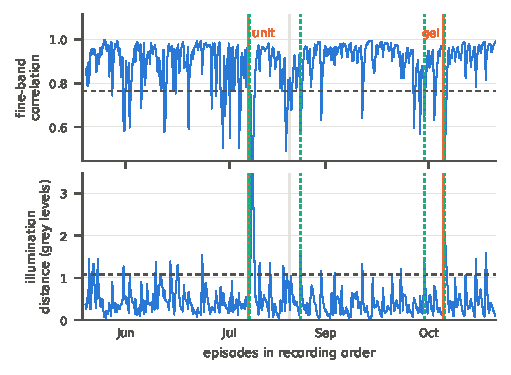
\includegraphics[width=\linewidth]{fig/fig_tracker.pdf}
  \caption{\textbf{\Cref{alg:tracker}'s detector over four months}, \EpRecorded\ episodes in recording order, on whole frames. Top: fine-band correlation between the last 8 episodes and the 30 before them. Bottom: distance between their illumination fields. Dashed: thresholds from the first hardware state. Orange: the change of unit and the gel replacement. Green: alarms (two false). Grey: the summer break.}
  \label{fig:tracker}
\end{figure}

\begin{table}[t]
  \centering\footnotesize\setlength{\tabcolsep}{3.5pt}
  \caption{\textbf{Detecting a change of hardware} with thresholds fixed in advance (10th and 95th percentiles of the two statistics on one unit of each dataset, $m\!=\!5$). Streams splice recordings of one unit or gel onto another (100 streams) or onto other recordings of the same hardware (100 streams). SITR: changes between two Minis only. Delay and false alarms are counted in the dataset's items.}
  \label{tab:detect}
  \resizebox{\linewidth}{!}{%
  \begin{tabular}{@{}llccc@{}}
    \toprule
    dataset & changes & detected & delay & false alarms \\
    & & (\pct) & (median) & per 1{,}000 \\
    \midrule
    ours, whole frames (episodes) & unit, gel & \TeOursFramesDet & \TeOursFramesDelay & \TeOursFramesFa \\
    ours, material crops (episodes) & unit, gel & \TeOursDet & \TeOursDelay & \TeOursFa \\
    SITR~\cite{sitr2025} (images) & Mini to Mini & \TeSitrMiniDet & \TeSitrMiniDelay & \TeSitrFa \\
    FEATS~\cite{feats2025} (images) & unit, gel & \TeFeatsDet & \TeFeatsDelay & \TeFeatsFa \\
    Tactile MNIST~\cite{tactilemnist2025} (touches) & gel & \TeTmnistDet & \TeTmnistDelay & \TeTmnistFa \\
    \bottomrule
  \end{tabular}}
\end{table}

Run over all \EpRecorded\ episodes in recording order (\cref{fig:tracker}), the detector raises \FrAlarms\ alarms. One comes \FrUnitLatency\ episodes after the change of unit and one \FrGelLatency\ episodes after the gel replacement. The other \FrFalseAlarms\ are false: one in the second September session, after the summer break, and one the day before the gel replacement. With stricter thresholds, the 1st and 99th percentiles, it detects both changes later (\FrSweepOneUnit\ and \FrSweepOneGel\ episodes) and raises no false alarm (supplement). A canvas session, whose weave lowers the fine correlation, and the illumination steps between sessions raise no alarm, because they do not occur together. \Cref{tab:detect} applies the same rule to streams spliced from four datasets, with thresholds set on one unit of each and nothing tuned on change points. It detects \TeOursFramesDet\pct\ of the changes spliced from our recordings: \TeOursFramesUnitDet\pct\ of those that involve the other unit, and \TeOursFramesGelDet\pct\ of the gel changes on the same unit. On the public datasets it detects \TePubDetMin--\TePubDetMax\pct, with \TePubFaMax\ or fewer false alarms per 1{,}000 items everywhere. Whole frames matter. Our first implementation computed the statistics on the material crops, which cover each frame sparsely, so that a window holds one object seen through a few crops per pixel. On the real stream it missed the change of unit, and on spliced streams it detected only \TeOursDet\pct\ of the changes. A per-object variant on the crops did no better (supplement). We moved to whole frames after these failures and kept the rule, so the real-stream result above is not an independent test, while the spliced public streams are.

Detecting the changes matters. A running mean that is never restarted reaches \SrcSupNoResetAcc\pct\ for the CNN. The crop-based detector missed the change of unit, so its estimate for the September sessions still averaged objects seen on the first unit, and the CNN reached \SrcSupTrkAcc\pct. With the whole-frame detector's restarts it reaches \SrcSupTrkFrAcc\pct. Started at the deployment in September, the reading gives \SrcSupTrkFrDepAcc\pct\ with the two false alarms and \SrcSupTrkDepAcc\pct\ with a single restart at the gel replacement, so the false alarms cost nothing measurable.

\subsection{What the estimate needs}
\label{sec:sources}

\begin{table}[t]
  \centering\footnotesize\setlength{\tabcolsep}{4pt}
  \caption{\textbf{Which estimate of the state} (accuracy on campaign D, three seeds). Every estimate uses unlabelled frames of the deployment.}
  \label{tab:sources}
  \begin{tabular}{@{}lcc@{}}
    \toprule
    estimate $\hat F$ subtracted from the test image & CNN & + jitter \\
    \midrule
    none & \SrcSupNoneAcc & \SrcAugNoneAcc \\
    previous session, mean in feature space & \SrcSupFeatAcc & \SrcAugFeatAcc \\
    previous session, mean colour only & \SrcSupMeancolAcc & \SrcAugMeancolAcc \\
    previous session, smooth illumination only & \SrcSupLowpassAcc & \SrcAugLowpassAcc \\
    previous session, full field & \SrcSupPrevAcc & \SrcAugPrevAcc \\
    own session's other contacts (same object) & \SrcSupOwnAcc & \SrcAugOwnAcc \\
    a random other session of the campaign & \SrcSupRandAcc & \SrcAugRandAcc \\
    all sessions of the campaign (non-causal) & \SrcSupCampAcc & \SrcAugCampAcc \\
    the session's bare gel & \SrcSupBlankAcc & \SrcAugBlankAcc \\
    \cref{alg:tracker} (causal, automatic restarts) & \SrcSupTrkFrAcc & \SrcAugTrkFrAcc \\
    \bottomrule
  \end{tabular}
\end{table}

\Cref{tab:sources} varies only the test-time estimate. Any unlabelled frames of the deployment work, provided they come from other objects: the previous session, a random other session, all sessions together, or the bare gel. The session's own contacts are the worst full-field estimate, because their mean contains the object. The number of objects matters more than the number of contacts. In a separate run with one seed, an estimate built from one other object gives \CvSupObjOne\pct, from two objects \CvSupObjTwo\pct\ and from nineteen \CvSupObjNineteen\pct. For the CNN, the smooth illumination field alone does as well as the full field (\SrcSupLowpassAcc\ against \SrcSupPrevAcc\pct). For the jitter CNN the fine pattern adds about four points (\SrcAugLowpassAcc\ against \SrcAugPrevAcc\pct). A single colour per session recovers part of the gain, and centring the features does not work. The bare gel works as well as the contacts, so standard flat-fielding is a valid estimate of the state where blank frames exist. The contact stream gives the same estimate where they do not, which is the case for archived datasets and for our training campaigns.

\subsection{Where the correction helps}
\label{sec:timeorstate}

\begin{table}[t]
  \centering\footnotesize\setlength{\tabcolsep}{3.5pt}
  \caption{\textbf{Each campaign held out in turn} (accuracy, 20-way). A and B are tested on hardware seen in training for every test material. In C, four test materials were learned on the other gel and wood on the other unit. D is the split of \cref{tab:material}. Folds A--C: one training seed.}
  \label{tab:rotation}
  \begin{tabular}{@{}lcccc@{}}
    \toprule
    test campaign & A & B & C & D \\
    \midrule
    CNN, raw & \FoldASupRawAcc & \FoldBSupRawAcc & \FoldCSupRawAcc & \SrcSupNoneAcc \\
    \ \ $-$ previous session's state & \FoldASupPrevAcc & \FoldBSupPrevAcc & \FoldCSupPrevAcc & \SrcSupPrevAcc \\
    CNN + jitter, raw & \FoldAAugRawAcc & \FoldBAugRawAcc & \FoldCAugRawAcc & \SrcAugNoneAcc \\
    \ \ $-$ previous session's state & \FoldAAugPrevAcc & \FoldBAugPrevAcc & \FoldCAugPrevAcc & \SrcAugPrevAcc \\
    Sparsh-I-JEPA, raw & \FoldAIjepaRawAcc & \FoldBIjepaRawAcc & \FoldCIjepaRawAcc & \IjepaRawAcc \\
    \ \ $-$ previous session's state & \FoldAIjepaPrevAcc & \FoldBIjepaPrevAcc & \FoldCIjepaPrevAcc & \IjepaPrevAcc \\
    \bottomrule
  \end{tabular}
\end{table}

\Cref{tab:rotation} holds out each campaign in turn. Time alone is not the problem. Sessions recorded weeks apart on the hardware seen in training are recognised at \FoldBSupRawAcc--\FoldASupRawAcc\pct\ raw (folds A and B), and the state itself changes little over three months. Its fine band still correlates at \HwFarMonths, against \HwFarWeeks\ after weeks, and its illumination field has moved by \LpDistStwoJulSep\ grey levels. Within known states the subtraction is unnecessary and can cost up to \num{10} points, because the training mean $G$ is then a mixture of states that no real session has. The gain in fold D is a gain against a collapse, and the collapse comes from the training set. Trained on A and B alone, which hold fifteen materials, all on unit 1, the CNN collapses less on D (\TsABSupRawAcc\pct\ raw over all 20 test materials, at most 75\pct\ possible, with \TsABSupRawTop\pct\ in one class). The state estimate adds less (\TsABSupPrevAcc\pct), and the jitter CNN gains nothing from it (\TsABAugRawAcc\ against \TsABAugPrevAcc\pct). Trained on A and C, with four materials again recorded only on unit 2, it collapses again (\TsACSupRawAcc\pct) and recovers to \TsACSupPrevAcc\pct. Trained on June alone, it scores \GapFoneSupBRawAcc\pct\ on its fifteen materials weeks later on the same unit and \GapFoneSupDRawAcc\pct\ on the other unit, and the estimate does not recover that loss (\GapFoneSupDPrevAcc\pct). The estimate therefore repairs the shortcut that one session per object creates, and it does not repair everything a change of hardware costs.

Two cases are not repaired. In fold C, all five test materials were learned on gel 3 only and are tested on earlier hardware. The four rigid materials score \FoldCSupRawFour\pct\ raw and \FoldCSupPrevFour\pct\ with the state removed, wood scores \FoldCSupRawWood\ and \FoldCSupPrevWood\pct, and frozen Sparsh is at chance. In fold D, the same four materials cross the gel replacement in the other direction, and the reading halves their accuracy. Wood, which crosses both unit and gel in fold D, is recovered there. Both failures involve the gel replacement. The change of unit also replaced a gel and was corrected, however, and the four materials are rigid and were recorded in a single session per gel. All sessions on the replaced gel hold these materials, so we cannot separate the gel, the materials and the training-set structure as the cause.

\subsection{Other sensors and the hardware in foundation features}
\label{sec:second}

\paragraph{Foundation features encode the unit.}
Fourteen materials were recorded on both units. A linear probe trained on frozen features of some of these materials, and tested on the others, tells the two units apart from a single crop at \ProbeSdinoRawUnit\pct\ for Sparsh-DINO, \ProbeIjepaRawUnit\ for Sparsh-I-JEPA, \ProbeDinovRawUnit\ for DINOv2 and \ProbeCnnRawUnit\ for our CNN, where chance is 50\pct. Read relative to the previous session's state, the same crops give \ProbeSdinoPrevUnit, \ProbeIjepaPrevUnit, \ProbeDinovPrevUnit\ and \ProbeCnnPrevUnit\pct, while the material probe on the same features drops by one to six points (supplement). The two units were also used in different seasons, which this probe cannot separate from the hardware.

\paragraph{SITR: four GelSight Minis.}
SITR's released classification set has 20 objects pressed on seven sensors, four of them GelSight Minis~\cite{sitr2025}. Following its protocol with a frozen DINOv2, a head trained on one Mini scores \SitrDinovRawIntra\pct\ on the other three raw, \SitrDinovBgIntra\pct\ with SITR's background image subtracted, and \SitrDinovStreamIntra\pct\ relative to the mean of the sensor's own unlabelled images. That mean uses the 16{,}000 images of the sensor's training split, and the test images are not among them. The mean of 100 random images gives \SitrDinovStreamHundredIntra\pct, and the mean of 20 is worse than no correction (\SitrDinovStreamTwentyIntra\pct), because it still contains the objects in those 20 presses. The stream estimate thus needs many images, while SITR needs 18 calibration presses per sensor. The hardware remains decodable after the correction (probe \SitrDinovStreamProbe\pct), and the reading does little for our CNN (\SitrCnnRawIntra\ to \SitrCnnStreamIntra\pct) or for Sparsh (\SitrIjepaRawIntra\ to \SitrIjepaStreamIntra\pct, supplement). SITR itself reports 90\pct\ on its 16-object version with calibration presses and simulated pretraining, and 73\pct\ for an ImageNet ViT.

\paragraph{FEATS: force across units and gels.}
FEATS records indenters with known force maps on five Minis and six gels~\cite{feats2025}. A linear probe on its labelled no-contact frames identifies both the sensor and the gel at \FeatsProbeSensor\pct, so the state is in the bare frame there as well. A CNN regressing normal force reaches \FeatsRawTestMae\,N on the training hardware and \FeatsRawOldGelMae\,N and \FeatsRawNewGelMae\,N on another unit with its old and a new gel. Relative to the stream estimate the errors are \FeatsStreamOldGelMae\ and \FeatsStreamNewGelMae\,N, and relative to the no-contact frame \FeatsBgOldGelMae\ and \FeatsBgNewGelMae\,N. No image-space reading brings force across hardware close to the training error.

\paragraph{Real Tactile MNIST: a gel swap on another lab's sensor.}
On Real Tactile MNIST (a digit from single touches, 24 runs over three weeks, one gel swap)~\cite{tactilemnist2025}, frozen Sparsh-I-JEPA collapses on later runs whether or not the gel was swapped, with \TmLaterIjepaRawTop\pct\ of the touches in one class on the same gel and \TmGelIjepaRawTop\pct\ after the swap. Reading relative to the previous run's state reduces the collapse in both cases and lifts accuracy from \TmLaterIjepaRawAcc\ to \TmLaterIjepaPrevAcc\pct\ and from \TmGelIjepaRawAcc\ to \TmGelIjepaPrevAcc\pct. The data therefore show the shortcut but do not tie it to the gel swap. For the supervised model, per-run AdaBN does better than the state reading (\TmGelSupAdaRunAcc\ against \TmGelSupPrevAcc\pct\ after the swap), because every run contains all ten digits. This is the mixed-class condition that our one-object sessions lack.

\subsection{Normal force}
\label{sec:force}
Force is a matter of mechanics, and the state does not describe it. Whole-frame models trained on June and July to regress normal force from appearance reach $R^2\le\ForceLearnedBestR$ on September and October, even with the state removed. Marker spreading measured against a bare-gel marker grid transfers better. June and July have no bare-gel frames, so their marker displacements are referenced to a bare-gel grid recorded in September. A linear map of three affine statistics of the displacement field, fitted on June and July, then predicts the September and October sessions before the gel replacement at $r=\ForceGeomXeraC$ ($R^2=\ForceGeomXeraR$), and the reverse fit predicts June and July at $r=\ForceGeomXeraRevC$. Within September and October, a fit on the first 13 sessions predicts the last 7, five of them on the replaced gel, at $R^2=\ForceGeomFreshR$ when each session uses its own bare-gel grid. Contact needs the unloaded gel as well. A detector that compares the embedding with the session's own bare gel rejects \ContactRefSpec\pct\ of other sessions' bare-gel frames, against \ContactRawSpec\pct\ without that reference, and plain differencing against the bare gel does about as well (\ContactBlankdiffSpecMin--\ContactBlankdiffSpecMax\pct, supplement).
